\documentclass[defaultpackages]{simplereport}
\usepackage{float}
\usepackage{listings}
\usepackage[]{enumitem}
\usepackage{bm}
\usepackage{tikz}
\usetikzlibrary{arrows,automata,positioning}
\title{Oblig 2}
\author{Åsmund Aqissiaq Arild Kløvstad}
\course[INF210]{Modelling of Computing}

\newcommand{\Z}{\mathbb{Z}}
\newcommand{\N}{\mathbb{N}}
\newcommand{\R}{\mathbb{R}}
\newcommand{\Q}{\mathbb{Q}}
\newcommand{\C}{\mathbb{C}}
\newcommand{\powerset}[1]{\mathcal{P}(#1)}
\newcommand{\gen}{\rightarrow^*}

\lstset{
  basicstyle=\itshape,
  xleftmargin=3em,
  mathescape,
  literate={->}{$\rightarrow$}{2}
           {l}{$\lambda$}{1}
}

\begin{document}
\maketitle{}
\section*{main.pdf 5.7}
\paragraph{\textbf{4)}} This exercise is about the language of balanced
parentheses \[D = \{\mathbf{u} \in \Sigma^* \mid \text{all prefixes contain at
  least as many ['s as ]'s, and the total number of ['s equal the number of ]'s}\}\]
\begin{itemize}[label=]
  \item \textbf{a)} List all words in $D$ of length 6.\\ There are 5:
    $[ [ [ ] ] ], [ ] [ [ ] ], [ [ ] ] [ ], [ [ ] [ ] ] \text{ and } [ ] [ ] [
    ]$.
    
  \item \textbf{b)} Show that the language of all words of $D$ with length at
    most $n$ is regular for any fixed $n$.\\
    All finite languages are regular since they can be constructed by a finite
    number of concatenations and unions of singleton languages. This language is finite and therefore
    regular.
    
  \item \textbf{c)} Is the Dyck language of depth at most 3 regular? (Depth is
    the maximal number of nested parentheses)\\
    This restricted language is recognized by the following finite automaton:
  \begin{figure}[H]
     \centering
     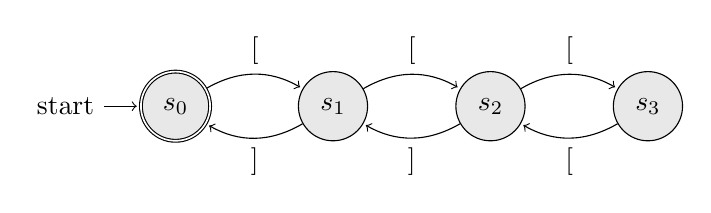
\begin{tikzpicture}[shorten >=1pt,node distance=2cm,on grid,auto]
       \tikzstyle{every state}=[fill={rgb:black, 1;white,10}]

       \node[state, initial, accepting] (s_0)                {$s_0$};
       \node[state]          (s_1) [right of=s_0] {$s_1$};
       \node[state]          (s_2) [right of=s_1] {$s_2$};
       \node[state]          (s_3) [right of=s_2] {$s_3$};

       \path[->]
       (s_0) edge [bend left] node {[} (s_1)
       (s_1) edge [bend left] node {[} (s_2)
             edge [bend left] node {]} (s_0)
       (s_2) edge [bend left] node {[} (s_3)
             edge [bend left] node {]} (s_1)
       (s_3) edge [bend left] node {[} (s_2);
     \end{tikzpicture}
  \end{figure}
  Since it is recognized by a finite automaton, it is regular.
  
\item \textbf{d)} Is the Dyck language of depth at most $n$ for any fixed $n$
  regular?\\
  We can construct a finite automaton like the one above for any fixed $n$ with
  $n+1$ states. By the same argument as before, this language is also regular.

\item \textbf{e)} Is the Dyck language regular?\\
  No. The language consisting of simply nested parentheses $\{[^n]^n \mid n \in \N\}$ is contained in
  the Dyck language. This is isomorphic to $\{a^nb^n \mid n \in \N\}$ which is
  known to be non-regular so the Dyck language is also non-regular.

\item \textbf{f)} An inductive definition of the Dyck language is given by:
  \[\lambda \in D'\]
  \[\mathbf{u}, \mathbf{v} \in D' \implies \mathbf{uv} \in D'\]
  \[\mathbf{w} \in D' \implies [\mathbf{w}] \in D'\]
  Show that these two definitions are equal.\\\\

  We will show the equality in two steps. First $D' \subseteq D$ by induction on
  the length of words $k$. As a base step for $k=0$, $\lambda \in D$ and also in
  $D'$ by definition. We form the induction hypothesis $\lvert \mathbf{w} \rvert
  \leq k,  \mathbf{w} \in D' \implies \mathbf{w} \in D$. Now we assume it holds for $k-1$ and
  show it also holds for $k$.\\
  Consider $\mathbf{w} \in D'$ of length $k$. Since it is in $D'$, either
  $\mathbf{w} = [\mathbf{w'}]$ or $\mathbf{w} = \mathbf{uv}$ for some
  $\mathbf{u,v, w'} \in D'$. In the first case $\lvert \mathbf{w'} \rvert \leq
  k$, so $\mathbf{w'}$ is in $D$ by the induction hypothesis and so $\mathbf{w}$
  is as well. In the second case $\lvert \mathbf{u} \rvert, \lvert \mathbf{v}
  \rvert < k$ (since we have used the rule to construct $\mathbf{w}$ from
  smaller parts) and hence in $D$ by the induction hypothesis. Since both are in
  $D$, they have an equal number of opening and closing parentheses, and so does
  $\mathbf{w}$ so it is in $D$.\\\\

  Secondly we show $D \subseteq D'$. First note that we can determine if a word
  is in $D$ by maintaining a counter as we read from left to right. Start the
  counter at 0, increase by one for each $[$ and decrease by one for each $]$.
  If this counter always remains non-negative and is 0 at the end of the word,
  then the word is in the Dyck language.
  \\
  First we look at a word $\mathbf{w}$ in $D$ such that the counter always
  monotonically increases, then monotonically decreases to 0. (This corresponds to
  simply nested parentheses.)
  Looking at the sequence of counter values we can reconstruct the word by
  concatenating a $[$ whenever it increases, and a $]$ whenever it decreases.
  For a  sequence that increases $n$ times and then decreases $n$ times, this
  construction is like taking $[\mathbf{w}]$ $n$ times and so the word is in
  $D'$ as well.\\

  Now we let the counter decrease to 0. If it ever reaches 0 after $i$ steps,
  then we know $\mathbf{u} = w_0...w_i \in D$ and by the preceding argument also in $D'$.
  Since the whole word is in $D$ it must again decrease to 0 and so $\mathbf{u}
  = w_{i+1}...w_n$ is also in $D'$ and by construction $\mathbf{w} =
  \mathbf{uv}$ is in $D'$ as well.\\

  This argument is not entirely complete since we could have words like $[[][]]$
  in which the counter is neither going straight up and down, nor reaching 0 in
  the middle. However we note that $[][]$ is covered by the second possibility
  and we can therefore surround it by parentheses and still have a word in $D'$.
\end{itemize}

\paragraph{\textbf{5)}} In this exercise we are asked to show that two PDA models
  are equivalent by showing each model \textit{emulates} the other. $M = (\Sigma,
  \Gamma, Q, q_0, \Delta, F)$ is as defined in the textbook and $M' = (\Sigma',
  \Gamma', !, Q', q_0' \Delta')$ is a PDA with empty-stack acceptance and the
  designated start-of-stack symbol $!$.
  \\\\
  First we construct an $M'$ emulating $M$. Since the PDAs should recognize the
  same language $\Sigma' = \Sigma$. We want to store the execution of
  $M$ on the stack of $M'$ so $\Gamma' = \{s \gamma t \mid s,t \in Q, \gamma \in
  \Gamma\} \cup \{!\}$. Our construction will have two states $Q' = \{q_0', q_1'\}$
  where $q_0'$ is the starting state and $q_1'$ will serve as a faux final
  state. We define $\Delta$ in three steps:
  \begin{enumerate}
  \item First the pushing rules $(q_0', a, s \alpha r; t \beta r, q_0')$ for each $(s, a,
  \alpha ; \beta, t) \in \Delta, a \in \Sigma \cup \{\lambda\}$ and $r \in Q$.
  These rules emulate all the rules in $M$ that push something on the stack and
  store the current state on stack. $r$ serves as a fallback state. Note that
  $\alpha$ and $\beta$ may be the empty word.
  \item Second the popping rules $(q_0', a, s \gamma t; \lambda, q_0')$ for $(s, a,
  \gamma; \lambda, t) \in \Delta$. These rules emulate popping the symbol
  $\gamma$ from the stack and moving to a new state. Because of the fallback
  states added by the pushing rules and the non-determinism of our model we
  avoid getting stuck.
  \item Finally we add the rules $(q_0', a, s \gamma f; \lambda, q_1')$ for each $f
  \in F$ to move into our ``accepting'' state and the single rule $(q_1',
  \lambda, !; \lambda, q_1)$ to pop the bottom-of-stack symbol. Since execution
  is non-deterministic we will move to this ``accepting'' state with only $!$ on
  the stack when $M$ would move to a final state with an empty stack. Then we
  pop the bottom-of-stack marker and accept.
  \end{enumerate}
  Finally we construct an $M$ emulating a given $M'$. From lectures (CFL.pdf
  slide 13) we know that such an $M'$ can be reduced to a single state, so we
  may assume without loss of generality that $M'$ is such a reduced PDA. Rules
  in $\Delta'$ are given as triples omitting the state.
  \\\\
  Again we want to decide the same languages so $\Sigma = \Sigma'$. This time we
  need not store any extra information in the stack so $\Gamma = \Gamma'$ as
  well. Instead we need extra states to emulate pushing words, so $Q = \Gamma'
  \cup \{q_0\} \cup \{f\}$ where $q_0$ is the starting state and $f$ is a final
  state. To avoid confusion $q_\gamma$ denotes the state associated with the
  stack symbol $\gamma$.

  To emulate a rule $(l, \gamma'; \bm{\omega}) \in \Delta'$ with
  $\bm{\omega} = \omega_1...\omega_n$ we add the rule $(q_0, l, \gamma';
  \lambda, q_{\omega_1})$ to reach a ``pushing state'' and then $(q_{\omega_i},
  \lambda, \lambda; \omega_{i+1}, q_{\omega_{i+1}})$ for each symbol $\omega_i$.
  Finally the rule $(q_{\omega_n}, \lambda, \lambda; \lambda, q_0)$ moves us
  back to where we started. This set of rules emulates pushing a word by moving
  through a series of ``pushing'' states corresponding to the symbols of the
  word and pushing them one by one.\\
  If $\bm{\omega} = \lambda$ we have $(q_0, l, \gamma'; \lambda, q_0)$ instead.
  
  To emulate accepting with an empty stack we add the rules $(q_0, l, \lambda; \lambda, f)$ for each $(l, !;
  \lambda) \in \Delta'$. This moves us to a final state if $M'$ would pop the
  bottom-of-stack symbol. We also add $(q_0, l, \gamma; \lambda, f)$ for each
  $(l, \gamma; \lambda)$ in $\Delta'$ in case $M'$ is not well behaved and
  replaces $!$. Since execution is non-deterministic and the only place to go
  from $f$ is to pop symbols and stay in $f$ we will end up in $f$ with an empty
  stack only if $M'$ would have an empty stack.
\section*{Textbook 3.3}
  Exercise 3) and 4) use the procedure described by the text book in section 3.3
  to mark pairs of states that cannot be collapsed, and then collapsing the
  remaining pairs.
\begin{itemize}[label=]
\item \textbf{3)} with one step labelled "a" from s4 to s2\\\\
  Step one marks $\{s_0, s_2\}, \{s_0, s_4\}, \{s_1, s_2\}, \{s_1, s_4\}, \{s_2,
  s_3\}, \{s_3, s_4\}$.\\
  Step two marks $\{s_0, s_1\}$ and $\{s_0, s_3\}$. The final two pairs are not
  marked in step three and we collapse $\{s_1, s_3\}$ and $\{s_2, s_4\}$
  resulting in the minimal automata in figure \ref{fig:3.3.3a}.
  \begin{figure}[H]
     \centering
     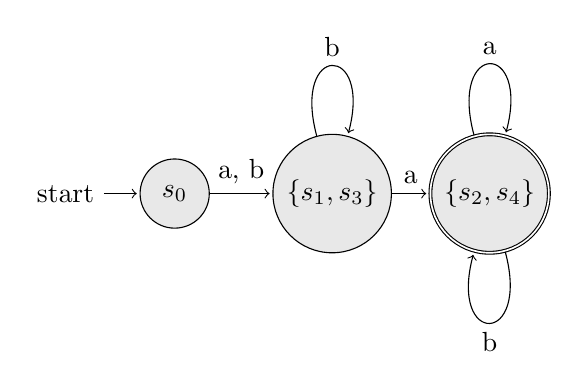
\begin{tikzpicture}[shorten >=1pt,node distance=2cm,on grid,auto]
       \tikzstyle{every state}=[fill={rgb:black, 1;white,10}]

       \node[state, initial] (s_0)                {$s_0$};
       \node[state]          (s_1) [right of=s_0] {$\{s_1, s_3\}$};
       \node[state,accepting](s_2) [right of=s_1] {$\{s_2, s_4\}$};

       \path[->]
       (s_0) edge [] node {a, b} (s_1)
       (s_1) edge [loop above] node {b} ()
             edge node {a} (s_2)
       (s_2) edge [loop above] node {a} ()
             edge [loop below] node {b} ();
     \end{tikzpicture}
     \caption{Minimal automata with ``a''-step from $s_4$ to $s_2$}
     \label{fig:3.3.3a}
  \end{figure}
\item \textbf{3)} as given\\\\
  This time all pairs are marked and no states can be collapsed.
  \begin{figure}[H]
     \centering
     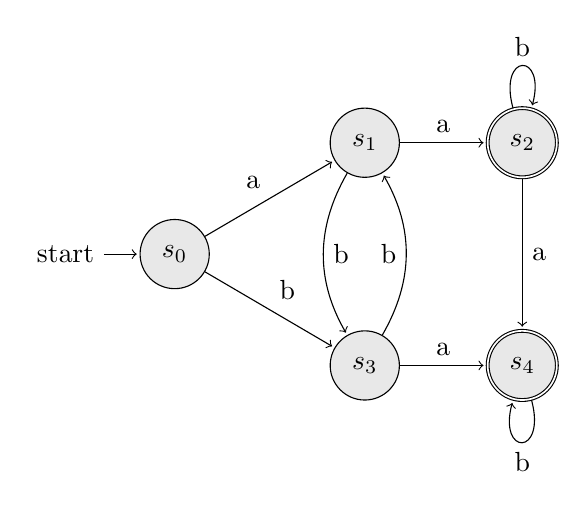
\begin{tikzpicture}[shorten >=1pt,node distance=2cm,on grid,auto]
       \tikzstyle{every state}=[fill={rgb:black, 1;white,10}]

       \node[state, initial] (s_0)                {$s_0$};
       \node[state]          (s_1) [above right of=s_0, xshift=1cm] {$s_1$};
       \node[state]          (s_4) [below right of=s_0, xshift=1cm] {$s_3$};
       \node[state,accepting](s_2) [right of=s_1] {$s_2$};
       \node[state,accepting](s_3) [right of=s_4] {$s_4$};

       \path[->]
       (s_0) edge [] node {a} (s_1)
             edge [] node {b} (s_4)
       (s_1) edge [bend right] node {b} (s_4)
             edge node {a} (s_2)
       (s_2) edge [loop above] node {b} ()
             edge [] node {a} (s_3)
       (s_3) edge [loop below] node {b} ()
       (s_4) edge [bend right] node {b} (s_1)
             edge [] node {a} (s_3);
     \end{tikzpicture}
     \caption{Minimal automata as given}
     \label{fig:3.3.3b}
  \end{figure}
 \item \textbf{4)}\\\\
  Step one marks $\{s_0, s_1\}, \{s_0, s_2\}, \{s_1, s_3\}, \{s_2, s_3\}$.\\
  Step two marks $\{s_1, s_3\}$ and $\{s_0, s_3\}$, so no pair of states can be
  collapsed. The FSM is minimal as given.

 \item \textbf{6)} Find minimal automaton for $a(b \mid c)^*bb^*$
  \begin{figure}[H]
     \centering
     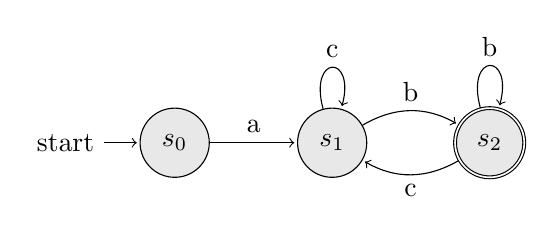
\begin{tikzpicture}[shorten >=1pt,node distance=2cm,on grid,auto]
       \tikzstyle{every state}=[fill={rgb:black, 1;white,10}]

       \node[state, initial] (s_0)                {$s_0$};
       \node[state](s_1) [right of=s_0] {$s_1$};
       \node[state,accepting](s_2) [right of=s_1] {$s_2$};

       \path[->]
       (s_0) edge [] node {a} (s_1)
       (s_1) edge [loop above] node {c} ()
             edge [bend left] node {b} (s_2)
       (s_2) edge [loop above] node {b} ()
             edge [bend left] node {c} (s_1);
     \end{tikzpicture}
     \caption{Minimal automaton for $a(b \mid c)^*bb^*$}
  \end{figure}
  To show this FSM is minimal we perform the same procedure as in 3) and 4).\\
  Step 1 marks $\{s_0, s_2\}$ and $\{s_1, s_2\}$, and $\{s_0, s_1\}$ cannot be
  collapsed since $\Upsilon(s_1, a)$ is not defined.
\end{itemize}
\section*{Textbook 3.4}
\begin{itemize}[label=]
  \item \textbf{6)} Determine whether the language $\{\mathbf{ww} \mid
    \mathbf{w} \in \Sigma^*, \lvert \Sigma \rvert = 2\}$ is regular.\\
    \\
    Assume regular. Then by pumping lemma there exists an $n > 0$ such that for
    any word $\mathbf{xyz}$ in the language of length $n$ or greater,
    $\mathbf{x}\mathbf{y}^k\mathbf{z}$ is also in the language for all $k$.\\
    Let $\mathbf{w} = 0^n1^n$ (with $\Sigma = \{0,1\}$, but isomorphic to any
    other such word over two letters). Now $\mathbf{ww}$ is certainly long
    enough for the pumping lemma and in the language by construction.
    Now let $\mathbf{ww} = \mathbf{xyz}$ in order to apply the pumping lemma.\\
    The pumping must occur within the first $n$ letters, so $\mathbf{xy}$ is a
    subword of $\mathbf{w}$ and $\mathbf{ww} = \mathbf{xyvw}$ for some $\mathbf{v}$.
    Then $\mathbf{xy}^0\mathbf{v}$ is either $a^{n-\lvert \mathbf{y} \rvert}b^n,
    a^nb^{n-\lvert \mathbf{y} \rvert}$ or $a^jb^k$ for some $j, k \neq n$.
    Either way $\mathbf{xy}^0\mathbf{v} \neq \mathbf{w}$ and $\mathbf{xy^0vw}$
    is not in the language and the pumping lemma does not hold.\\
    We conclude that the language is not regular.
  \item \textbf{7)} Determine whether the language $\{a^{2n} \mid n \geq 1\}$ is
    regular.\\\\
    We note that the language is described by the regular expression $(aa)^+$
    and conclude it is regular.
  \item \textbf{10)} Determine whether the language $\{\mathbf{ww}^R \mid
    \mathbf{w} \in \{a, b\}^*, \lvert \mathbf{w} \rvert \leq 3\}$ is
    regular.\\\\
    The language is finite, and therefore regular. It is described by the
    (exhaustive) regular expression ${aaaaaa} \mid {bbbbbb} \mid
    {abaaba} \mid {baaaab} \mid {aabbaa} \mid {abbbba} \mid {aaaa}
    \mid {bbbb} \mid {abba} \mid {baab} \mid {aa} \mid {bb} \mid \lambda$.
\end{itemize}
\section*{Textbook 3.5}
\begin{itemize}[label=]
  \item \textbf{1)} Prove there is an algorithm to decide if a regular language $L = \Sigma^*$\\\\
    We construct a 3-step algorithm based on the observation that $\Sigma^*
    \setminus \Sigma^* = \emptyset$
    \begin{enumerate}
    \item Construct a finite automaton $M_L$ accepting L
    \item Swap final and non-final states of $M_L$ to obtain an automaton for the complement of $L = \Sigma^* \setminus L$.
    \item For each final state in $M_{\Sigma^* \setminus L}$, check if reachable
      from initial state. If yes, then $L \neq \Sigma^*$. If no final states
      are reachable then $L = \Sigma^*$.
    \end{enumerate}
   This algorithm will terminate since $M_L$ is finite and hence $M_{\Sigma^*
     \setminus L}$ is finite. It produces the correct answer because $\Sigma^*
   \setminus L = \emptyset$ if and only if $L = \Sigma^*$
  \item \textbf{6)} Prove there is an algorithm for determining if there is a
    word in a regular language that begins with a given letter.\\\\
    Assume we have a finite automaton $M_L$ accepting $L$. Then for each state
    $q_i$ reachable from $q_0$ by the given letter and each final state $f_i$:
    if $f_i$ is reachable from $q_i$, return ``yes''. Then if we exhaust the
    search, return ``no''.\\
    This algorithm will terminate since $M_L$ is final. It gives the correct
    answer because any accepting path for a word starting with the given letter
    must start with that letter and end in a final state.
  \item \textbf{7)} Prove there is an algorithm to determine if a regular
    language contains a word of even length.\\\\
    We construct a 2-step algorithm based on the observation that any even
    number is a multiple of 2, and the assumption that we can find a path
    between two nodes in a graph. We also assume a finite automaton $M_L$
    accepting $L$:
    \begin{enumerate}
      \item construct a graph $G$ such that $V(G) = Q$ and $E(G) = \{(q_i, q_j)
        \mid \text{there is a path of length 2 from} q_i \text{to} q_j \text{in}
        M_L\}$
       \item for each final state $f_i$, check if it can be reached from $q_0$
         in G. 
      \end{enumerate}
   This algorithm gives the right answer because a final state can be reached
   from the start state in G iff a word of even length is accepted by $M_L$. To
   determine whether there is a path from $q_0$ to $f_i$ we can use a simple
   breadth-first search, requiring at most $\lvert {V} \rvert + \lvert {E}
   \rvert$ steps. Doing this naively for each $f_i \in F$ (where $F$ is the set
   of final states in $M_L$) results in at most $\lvert F \rvert (\lvert {V} \rvert + \lvert {E}
   \rvert)$ steps.
\end{itemize}
\section*{Textbook 3.6}
\begin{itemize}[label=]
  \item \textbf{18)} Construct a pushdown automaton accepting $L =
    \{\textbf{w}c\textbf{w}^r \mid \textbf{w} \in \{a, b\}^*\}$.\\\\
    Use PDA model with empty stack-acceptance and stack alphabet $\{\alpha, \beta\}$.
    \begin{figure}[H]
     \centering
     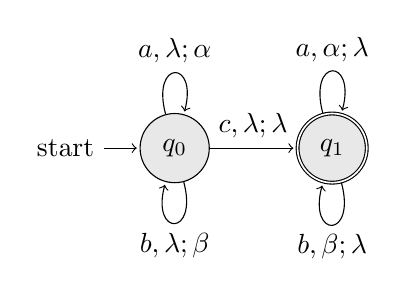
\begin{tikzpicture}[shorten >=1pt,node distance=2cm,on grid,auto]
       \tikzstyle{every state}=[fill={rgb:black, 1;white,10}]

       \node[state, initial] (s_0) {$q_0$};
       \node[state, accepting](s_1) [right of=s_0] {$q_1$};

       \path[->]
       (s_0) edge [loop above] node {$a,\lambda;\alpha$} ()
             edge [loop below] node {$b, \lambda; \beta$} ()
             edge [] node {$c, \lambda ; \lambda$} (s_1)
       (s_1) edge [loop above] node {$a,\alpha;\lambda$} ()
             edge [loop below] node {$b, \beta; \lambda$} ();
     \end{tikzpicture}
     \caption{pushdown automaton accepting $L = \{\textbf{w}c\textbf{w}^r \mid \textbf{w} \in \{a, b\}^*\}$}
   \end{figure}
   
   \item Show that the class of languages accepted by PDA's is closed under
     union, concatenation and and the Kleene star.\\\\
     We will show this by construction of new PDA's. Assume the PDA $M_L =
     \langle \Sigma, \Gamma, Q, q_0, \Delta, F \rangle$ accepts the language $L$
     and $M_{L'} = \langle \Sigma', \Gamma', Q', q'_0, \Delta', F' \rangle$
     accepts $L'$.\\

     First we construct a PDA which accepts $L \cup L'$. $M_{L \cup L'} =
     \langle \Sigma \cup \Sigma', \Gamma \cup \Gamma', Q \uplus Q' \cup \{q''_0\},
     q''_0, \Delta'', F \cup F' \cup \{q''_0\} \text{ if $q_0$ or $q'_0$ is final}
     \rangle$ where $\Delta'' = \Delta \cup \Delta' \cup \{(q''_0, a, \alpha ;
     \beta, q_i) \mid (q_0, a, \alpha ; \beta, q_i) \in Q \lor (q'_0, a, \alpha
     ; \beta, q_i) \in Q'\}$.
     That is a PDA whose alphabet and stack alphabet are simply the union of the
     original PDAs'. In the set of states take a disjoint union and add a new
     initial state $q''_0$. This is also in $F''$ if either original initial state was final.
     Finally we add rules to go from the new initial state to all states
     reachable from original initial states. This is straight-forwardly analogous to the
     construction of $M_{L \cup L'}$ for finite automata.\\
     This new PDA accepts all the words in $L$ because paths through $M_L$ are
     also in $M_{L \cup L'}$. It accepts the words in $L'$ by the same argument.
     It does not accept any other words because any path from $q''_0$ to a final
     state is also a path from either $q_0$ or $q'_0$ to a final state, with the
     first swapped for one of the new added steps and hence must be in $L$ or
     $L'$.\\

     
     To construct a PDA which accepts $L \cdot L'$ we ``append'' $M_{L'}$ to $M_L$. Let
     $$M_{L \cdot L'} = \langle \Sigma \cup \Sigma', (\Gamma \uplus \Gamma')
     \cup \{!\}, Q
     \uplus Q', \{q_o\}, \Delta'', F' \rangle$$ where $\Delta'' = \Delta \cup
     \Delta' \cup \{(q_i, \lambda, !; \lambda, q'_0) \mid q_i \in F\}$ and $!$
     is a new symbol to signify bottom of the stack. We start with this $!$ on
     the stack.\\
     This new machine is like executing $M_L$ and the, if we reach a final state
     with $!$ on the stack, popping $!$ and executing $M_L'$ on the remainder of
     the input. It accepts $L \cdot L'$

     Finally, the Kleene star of a language $L^*$ is accepted by ``looping''
     $M_L$. To do this we add a new initial and final state $q'_0$, a
     bottom of stack symbol $!$, and an ``empty'' rule $(q'_0, \lambda, \lambda;
     !, q_0)$, allowing our new machine to accept the empty word (zero loops)
     and pushing our bottom stack symbol before starting $M_L$. Then we add
     rules $\{(q_i, \lambda, !; \lambda, q'_0) \mid q_i \in F\}$ to go from any
     final state to the start state. These rules pop $!$ allowing for acceptance
     in $q'_0$ so we can remove them from $F$ leaving $q'_0$ as the only
     accepting state.
     
\end{itemize}
\section*{Textbook 4.1}
\begin{itemize}[label=]
  \item \textbf{14)} Construct a grammar for the language $(ab)^* \mid (ac)^*$
    \begin{lstlisting}
      S -> abA | acB
      A -> abA | l
      B -> acB | l
      \end{lstlisting}
  \item \textbf{21)} Construct a grammar for the language $(a | b)^*(aa | bb)(a|b)^*$
    \begin{lstlisting}
      S -> aA | bA | B
      A -> aA | bA | B
      B -> aaC | bbC
      C -> aC | bC | l
      \end{lstlisting}
   \item \textbf{24)} Find an automaton which accepts the language generated by
     \lstinline{S -> aB}, \lstinline{A -> aB}, \lstinline{B -> bA | b}\\\\
    We construct an automaton with states $N \cup \{f\}$ and initial state $S$
    following the procedure:
    \begin{itemize}[label=$\cdot$]
    \item \lstinline{A -> aB} becomes the rule $(A, a, B)$
    \item \lstinline{A -> a} becomes the rule $(A, a, f)$
      \item \lstinline{A -> l} makes $A$ final
      \end{itemize}
    \begin{figure}[H]
     \centering
     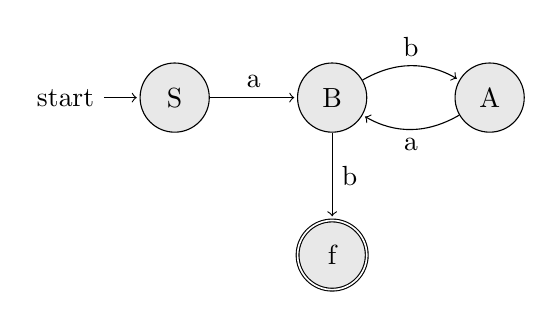
\begin{tikzpicture}[shorten >=1pt,node distance=2cm,on grid,auto]
       \tikzstyle{every state}=[fill={rgb:black, 1;white,10}]

       \node[state, initial] (S) {S};
       \node[state] (B) [right of=S] {B};
       \node[state] (A) [right of=B] {A};
       \node[state, accepting] (f) [below of=B] {f};

       \path[->]
       (S) edge [] node {a} (B)
       (B) edge [bend left] node {b} (A)
       edge [] node {b} (f)
       (A) edge [bend left] node {a} (B);
     \end{tikzpicture}
     \caption{The finite automaton for \textbf{24)}}
     \end{figure}
   \item \textbf{36)} Construct a grammar that generates the language accepted
     by a given finite automaton.\\\\
     We apply the procedure from the previous question in reverse.
     \begin{itemize}[label=$\cdot$]
      \item the rule $(Q, a, Q')$ becomes \lstinline{Q -> aQ'}
      \item if $Q' \in F$, add \lstinline{Q -> a} to our grammar rules
      \item if $Q \in F$, add \lstinline{Q -> l} to our rules
      \end{itemize}
      Also note that the state $S_4$ is a dead end, and will not contribute to
      the accepted language. The resulting grammar has $N = \{S_0, S_1, S_2,
      S_3\}$, $\Sigma = \{a, b\}$ and production rules:
      \begin{itemize}[label=]
      \item $S_0 \rightarrow aS_1 \mid bS_2$
        \item $S_1 \rightarrow bS_1 \mid aS_3 \mid a$
        \item $S_2 \rightarrow aS_1 \mid bS_3 \mid b$
          \item $S_3 \rightarrow \lambda$
        \end{itemize}
  \end{itemize}

  \section*{Textbook 4.2}
  \textbf{4)} and \textbf{5)} concern the grammar $G$ with $N = \{A, B, S\}$,
  $\Sigma = {a, b}$, $R:$
    \begin{lstlisting}
      S -> ABABABA
      A -> Aa | l
      B -> b
      \end{lstlisting}
  \begin{itemize}[label=]
  \item \textbf{4)} convert the grammar to Chomsky Normal Form (CNF).\\
    We proceed in 3 steps:
    \begin{enumerate}
      \item Remove \lstinline{A -> Aa} by constructing the new non-terminal
        $N_a$ and rules \lstinline{$N_a$ -> a, A -> A$N_a$}
      \item Eliminate rules with more than two non-terminals on the right. We
        replace \lstinline{S -> ABABABA} with
        \begin{lstlisting}
S -> A$S_1$
$S_1$ -> B$S_2$
$S_2$ -> A$S_3$
$S_3$ -> B$S_4$
$S_4$ -> A$S_5$
$S_5$ -> BA
        \end{lstlisting}
      \item Get rid of the null production \lstinline{A -> l}. We also have to
        add rules \lstinline{B -> X} for any existing rule \lstinline{B -> AX}
        or \lstinline{B -> XA}
      \end{enumerate}
      The resulting grammar $G' = \langle \Sigma, N \cup \{N_a, S_{1}, ... ,
      S_5\}, S, R' \rangle$ with $R' = $
      \begin{lstlisting}
A -> A$N_a$
$N_a$ -> a
B -> b
S -> A$S_1$
$S_1$ -> B$S_2$
$S_2$ -> A$S_3$
$S_3$ -> B$S_4$
$S_4$ -> A$S_5$
$S_5$ -> BA
A -> $N_a$
S -> $S_1$
$S_2$ -> $S_3$
$S_4$ -> $S_5$
$S_5$ -> B
\end{lstlisting}

    \item \textbf{5)} convert the grammar to Greibach normal form\\
      Starting with the grammar $G'$ already in CNF we proceed in two steps:
      \begin{enumerate}
        \item Remove the left recursive rule \lstinline{A -> A$N_a$} by
          replacing it with \lstinline{A -> A', A' -> aA'}
        \item Get rid of non-terminals on the left of productions by replacing
          them with the terminals they generate.
        \end{enumerate}
     We obtain a new grammar with $N'' = \{N \cup \{A', S_1 ... S_6\}\}$ and
     $R'' =$
     \begin{lstlisting}
$S$ -> aA'$S_1$ | b$S_2$
$S_1$ -> b$S_2$
$S_2$ -> aA'$S_3$ | b$S_4$
$S_3$ -> b$S_4$ | b$S_6$
$S_4$ -> aA'$S_5$
$S_5$ -> b | b$S_6$
$S_6$ -> a | aA'
$A$ -> a | aA' | l
\end{lstlisting}

   \item \textbf{8)} Convert the following grammar to CNF:
     \begin{lstlisting}
S -> AbaB
A -> bAa | l
B -> AAb | aabA
\end{lstlisting}
     Following the same procedure as exercise \textbf{4)} we obtain:
     \begin{lstlisting}
$N_a$ -> a
$N_b$ -> b
S -> A$S_1$ | $S_1$
$S_1$ -> $N_b S_2$
$S_2$ -> $N_a$B
A -> $N_b A_1$
$A_1$ -> A$N_a$ | $N_a$
B -> $B_1$ | A$B_1$ | $N_a B_2$
$B_1$ -> $N_b$
$B_2$ -> $N_a N_b$
\end{lstlisting}

   \item \textbf{9)} convert the preceding grammar to GNF
     This time there are no left-recursive rules to eliminate, so the only
     necessary step is replacing leading non-terminals with the terminals they
     generate. We note $A \gen bA_1, \; A_1 \gen b A_1 a | a, \; B_1 \gen
     bA_1N_b, \;B_2 \gen ab,\; N_a \gen a, \; N_b \gen b$ and construct the production rules:
     \begin{lstlisting}
$N_a$ -> a
$N_b$ -> b
S-> b$A_1 B_1$ | b $S_2$
$S_1$ -> b$S_2$
$S_2$ -> aB
A -> b$A_1$
$A_1$ -> B$A_1 N_a$ | a
B -> b$A_1 B_1$ | a$B_2$ | b$A_1 N_b$ | b
$B_1$ -> b$A_1 N_b$ | b
$B_2$ -> a$N_b$
\end{lstlisting}
   \end{itemize}
\end{document}
